\chapter{Privacy and security}
\label{ch:security}

Punchscan intends to provide two measures of security: Voters' privacy and vote
integrity. This chapter will show to what extend it succeeds in doing that, and
what its limitations are.

\section{Voter privacy}

Voter privacy is essential to prevent a malicious third party from buying, or
coercing, voters. It is clear that privacy can not be guaranteed by the voting
system alone: Consider the case of a voter filming themselves during the voting
process. However a voting system should be able to ensure that, after the
voting process, a voter's privacy cannot be violated anymore. Other risks to
voter privacy would have to be addressed by regulations, such as not
permitting the use of video-capturing devices in voting booths.

\subsection{Privacy against a malicious election authority}

Punchscan does not achieve any form of privacy against a malicious election
authority. Having full access to the \textbf{P} table means that they can
reconstruct any voter's plaintext vote. Assuming voting booth workers to be
compromised, this then leaks every voter's vote.

\subsection{Privacy against third parties}

After having voted, a voter is left with one half of the ballot. A third party
will then, at most, have access to the following:
\begin{itemize}
\item For every ballot, either \ptop{} or \pbottom{} due to the scanned receipts being published along with their ballot ID
\item For each shard of the \textbf{D} table, either the \pone{} or the \ptwo{}
permutations
\item For each shard of the \textbf{D} table, either the $ID_P$ link to the
\textbf{P} table, or the $ID_R$ link to the \textbf{R} table
\item The full results table
\end{itemize}

Thus they will, for any given ballot, be lacking one of the ballot
permutations, one of the decryption permutations, and one of the chain of
mappings from \textbf{P} to \textbf{D} to \textbf{R} tables. Hence they will not be
able to learn the plaintext vote of any ballot.

\subsection{Vote-buying attack}

There does however exist a vote-buying attack on an earlier version of
punchscan, described by Moran and
Naor\autocite{moranSplitballotVotingEverlasting2010}. The key difference is
that this earlier version of Punchscan did not require a voter to commit to
which half of the ballot to keep until after they had voted. It can be shown
that a coercing party can pick a subset of receipts for which they are willing
to pay in such a way as to influence the election outcome.

For illustration purposes consider a vote between two candidates, Alice and
Bob. There will be two choices for \ptop{}, two for \pbottom{}, leading to four
different ballots. Assume the coercing party wants to influence the vote in
favour of Alice. Assume they state that they will pay for any ballot receipt,
as long as:
\begin{itemize}
\item It is not a ballot where the order of options is $b \rightarrow a$
\item And the voter did not selection the second option
\end{itemize}

The four possible ballots, with their respective ballot halves, are shown in
figure \ref{fig:vote_buying}. Green ballot halves are those with order $a
\rightarrow b$, so a voter will receive payment no matter who they vote for.
Orange ones are $b \rightarrow a$ receipts, so the voter must pick the left
option --- voting for Bob --- if they want to get paid. Red ones are $b
\rightarrow a$ receipts, so the voster must vote for Alice in order to get paid.
Thus the coercing party is able to force one out of four Bob voters to vote for
Alice, without causing any Alice voters to vote for Bob.

The same attack is also shown to be extensible to questions with more than two
votes. The fix for Punchscan is straight-forward, requiring voters to commit to
which half of the ballot to keep before they get access to the ballot. This way
the coercing party will also inadvertently pay Alice voters to vote for Bob
instead.

\begin{figure}
\centering
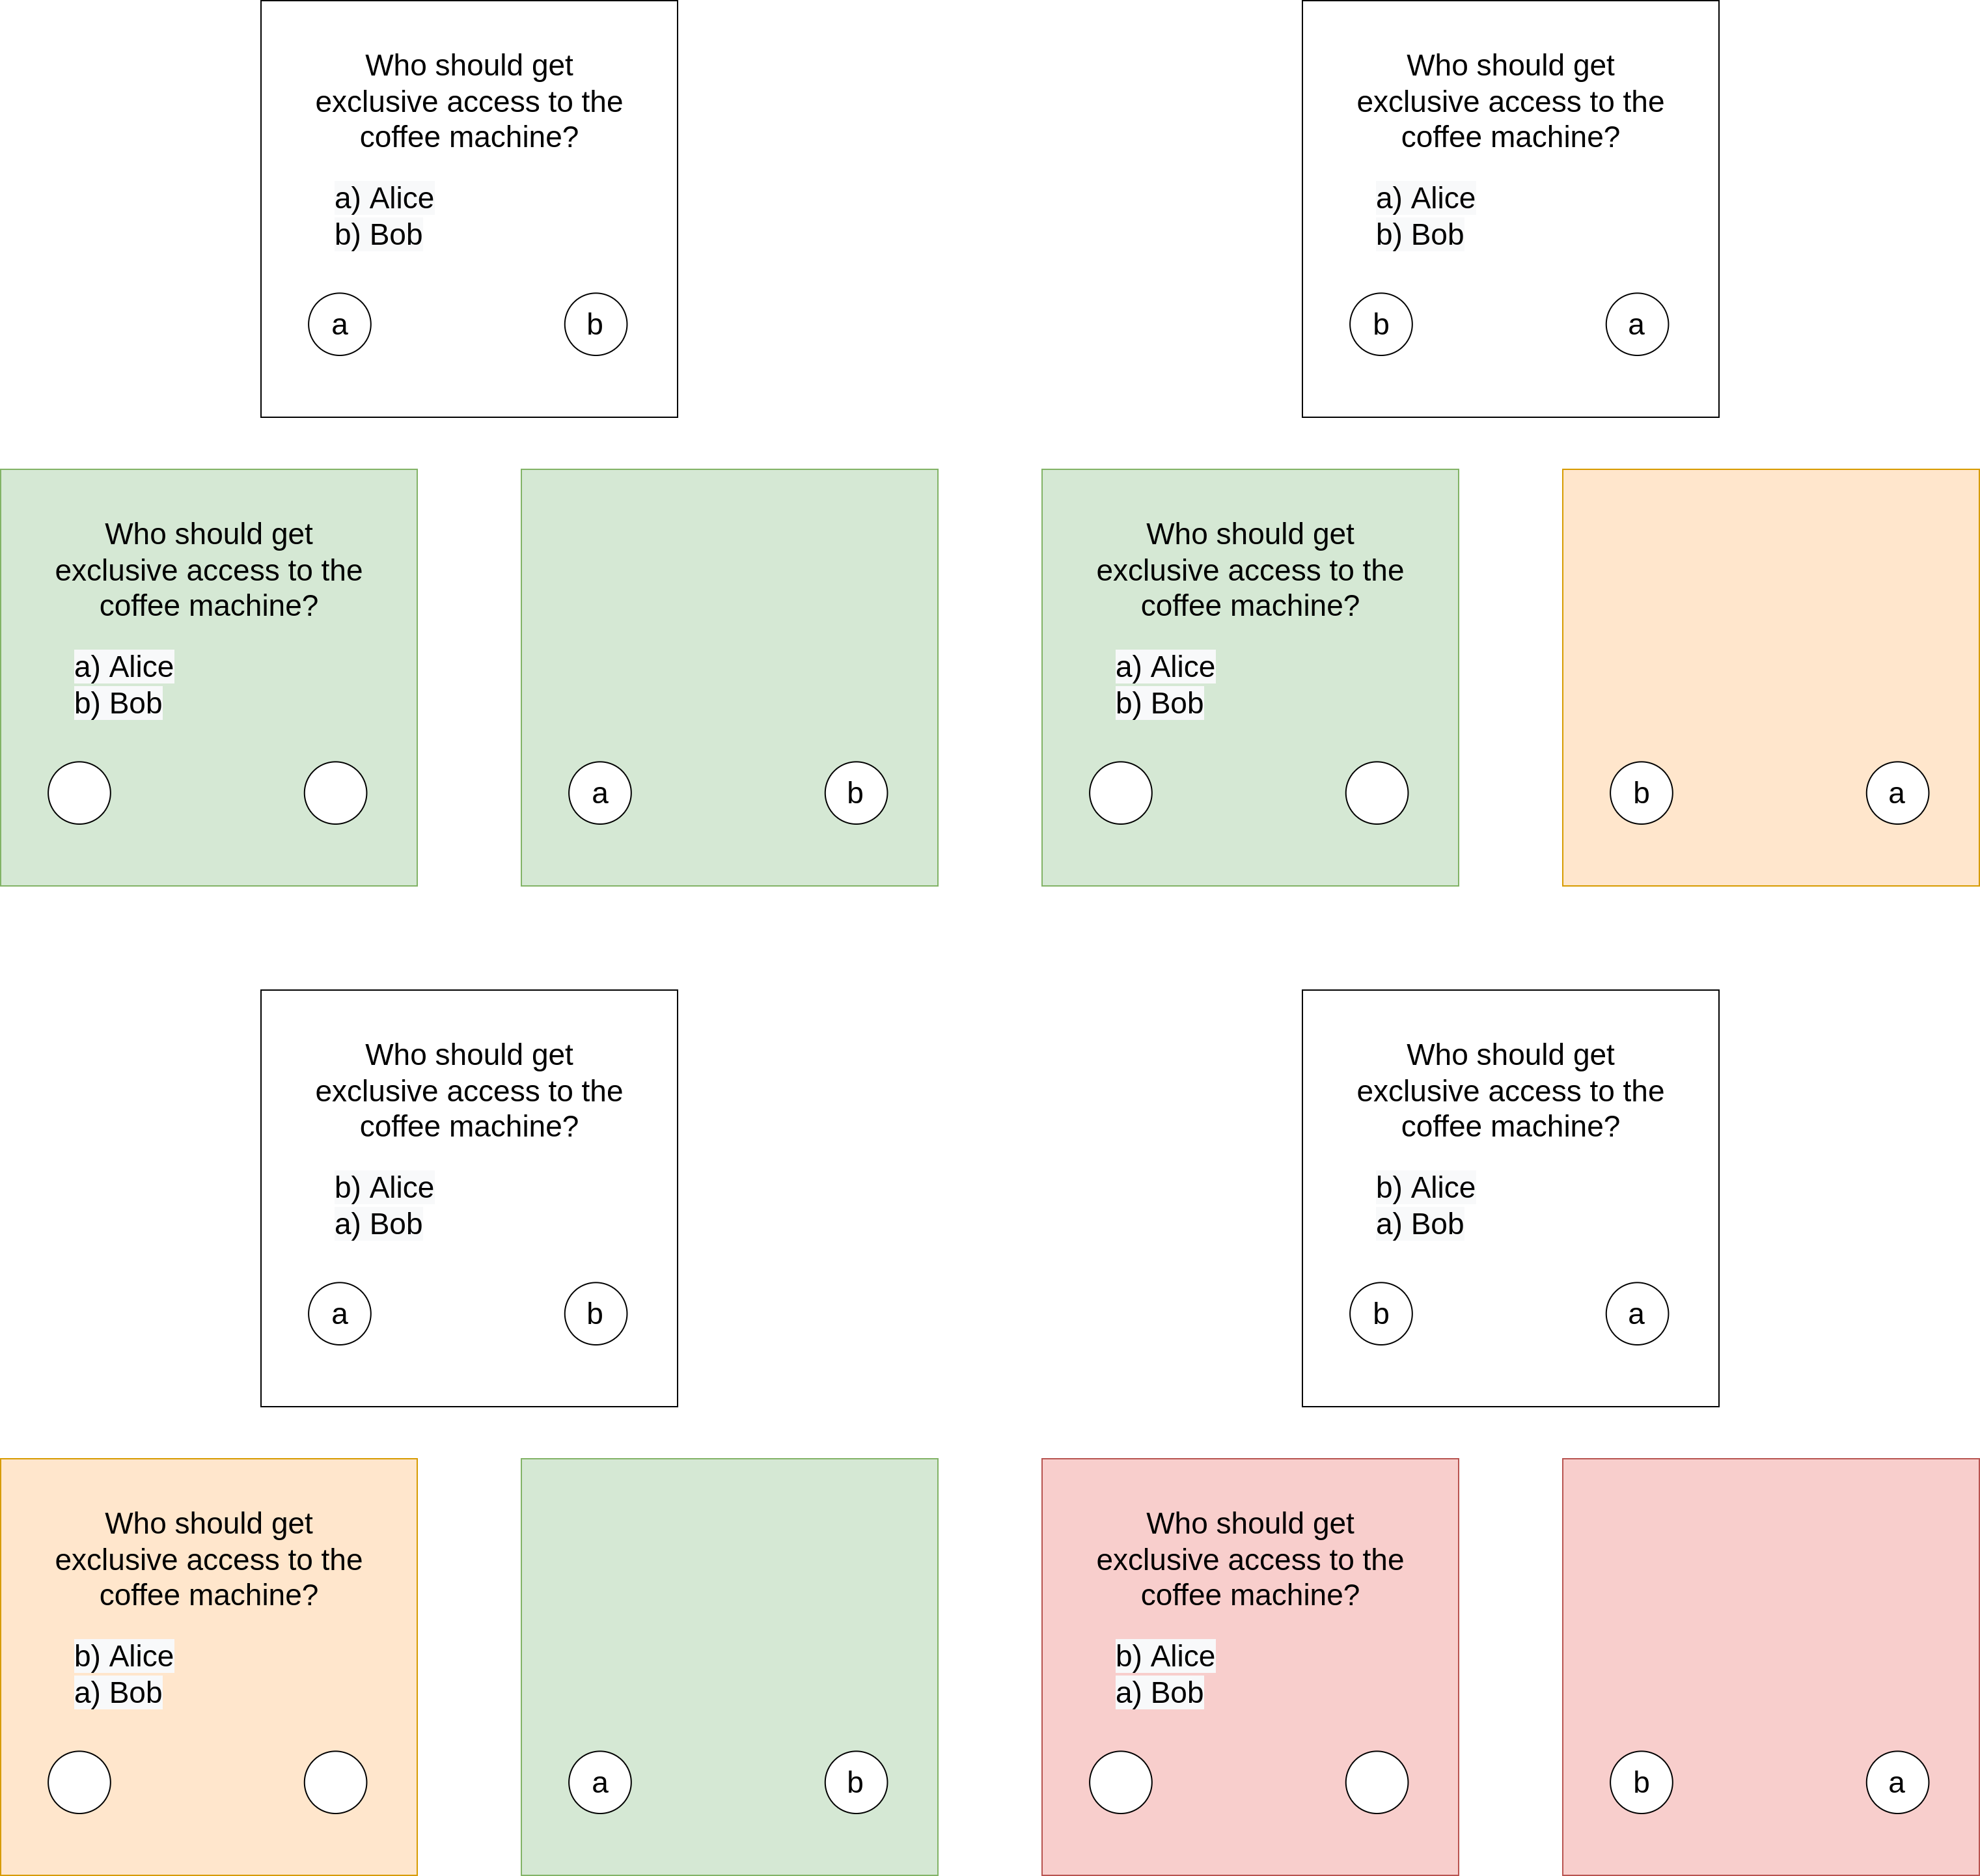
\includegraphics[width=0.8\textwidth]{../resources/vote_buying_split_highlighted_no_selection.drawio.png}
\caption{Green ballot halves allow getting paid no matter who you vote for. Orange ones require voting for Bob. Red ones require voting for Alice.}
\label{fig:vote_buying}
\end{figure}

\section{Vote integrity}

Punchscan provides some form of vote integrity versus a malicious election
authority --- at least during the setup and decryption phases.

\subsection{Setup-phase audit}

Recall that during the setup phase a certain number of rows of the \textbf{P} and
\textbf{D} tables are spoiled and verified. Thus for every row where the election authority 
was dishonest there is a chance of $\frac{1}{2}$ of it being caught. Consider the
generalized case where the election authority cheats on $f$ out of $n$ ballots,
with $k$ being audited. The introductory paper shows that an upper bound of the
election authority not being caught is given by:

\[
	[(1 - \frac{k}{n})^f, (1 - \frac{f}{n})^k]
\]

This bound can be made arbitrarily small by increasing the ratio of audited
ballots to total ballots.

\subsection{Decryption-phase audit}

Recall that during decryption one half of each shard of the \textbf{D} table is
revealed. To minimze its chance of being caught, a cheating election authority
will spread the votes on which it cheated across as few shards as possible.
Assuming $k$ shards were tempered with then this audit has a chance of
$\frac{1}{2^k}$ of not detecting this. Both this probability, as well as the
signifiance (in terms of tampered-with votes) of a single tampered-with shard
not being caught, can be lowered by decreasing the shard size. In the extreme
case one picks a shard size of $1$, at which points $k$ tampered votes have a
probability of $\frac{1}{2^k}$ of not being detected.

\subsection{Individual verifiability}

As the election authority publishes all scanned ballot receipts, any voter can
subsequently look up their receipt using their ballot ID. They can then compare
the scanned image with their physical receipt. This guarantees them that their
vote was at least cast-as-intended, although it does not ensure that it was
actually counted --- for this they must rely on the auditors having done their
job.

\subsection{Ballot misprinting}

One issue not addressed by Punchscan is the one of ballot integrity.
Fundamentally one must ensure that the printed ballots correspond to the the
remainders of the \textbf{P} table after the setup audit. The Punchscan paper
advises that voters should, the moment they receive the ballot, verify that
their ballot's commitment matches one of the published commitments. They do not
however provide any way in which a voter --- equipped with pen and paper ---
can do so in the few minutes they spend in a voting booth.

An alternative might be to introduce an additional audit phase, during which a
fraction of printed ballots is audited. The remaining unspoiled ballots would
then be sealed by the auditors, and not reopened until the day of the election.
No discussion of this takes place in the Punchscan paper, but Kelsyey et
al\autocite{kelseyAttackingPaperBasedE2E2010} mention it in passing.

\subsection{Malicious poll workers}

Kelsey et al also discuss a specific misprinting attack on
Punchscan\autocite[chapter 3]{kelseyAttackingPaperBasedE2E2010} where, when a
voter announced which half of the ballot they intend to keep, the poll worker
hands them a ballot where the half which will be destroyed is manipulated. As
discussed the voter is unable to verify the commitments in the voting booth.
When they then leave the voting booth, the only evidence of having cheated ---
the manipulated half of the ballot --- is destroyed. To prevent this one would
have to make poll workers commit to which ballot to hand out before the voter
announces which page to keep. At the same time one must still ensure that a
voter does not see their future ballot until after they commited to which half
to keep. Even more ways by which a cheating election authority can influence
the vote are discussed by Lundin et al\autocite{lundinTearDestroyChain2012}.

\section{Attacking cryptographic primitives}

The Punchscan paper goes into some detail to discuss potential attacks on the
cryptographic primitives they use for e.g. row commitments or the generation of
permutations. This will not be discussed here, as the security assumptions
placed on basic cryptographic primitives are assumed to hold.
